% !TeX encoding = utf-8
\documentclass[a4paper,12pt]{diplom}
\inputencoding{utf8}
\usepackage{paratype}
\DeclareMathSizes{12}{13.4}{11}{10}

\usepackage[left=3cm,right=2cm,top=2cm,bottom=2cm]{geometry} % Размеры полей
\usepackage[onehalfspacing]{setspace} % Полуторный интервал
%\renewcommand{\baselinestretch}{1.25} % Полуторный интервал
\usepackage{indentfirst} % Абзацный отступ в начале разделов
\setlength{\parindent}{1.25cm} % Величина абзацного отступа

\usepackage[pdftex]{graphicx} % Для вставки изображений
\usepackage{array} % Для таблиц
\usepackage{booktabs} % Для красивых таблиц 
\usepackage{tikz} % Рисунки с помощью TikZ
\usepackage[linesnumbered,lined,ruled]{algorithm2e} % Для оформления псевдокода
%\usepackage{algorithm} % Альтернатива оформления псевдокода
%\usepackage{algpseudocode} % Альтернатива оформления псевдокода
\usepackage{listings} % Оформление листингов программ
\usepackage{icomma} % Удаляем тонкий пробел после запятой в мат. режиме

% Если на нумерованную формулу нет ссылки в тексте,
\mathtoolsset{showonlyrefs} % то она становится ненумерованной

% microtype улучшает распределение символов в строке
\usepackage{microtype}  % Можно отключить, если возникают ошибки компиляции

% Формируем PDF с полноценными перекрестными ссылками
\usepackage[unicode, pdfborder={0 0 0}, pdfstartview=FitV]{hyperref}

% Часто используемые макросы
\newcommand{\N}{\mathbb{N}}  % Множество натуральных чисел
\newcommand{\Z}{\mathbb{Z}}  % Множество целых чисел
\newcommand{\R}{\mathbb{R}}  % Множество действительных чисел
\DeclareMathOperator{\sgn}{sgn} % Знак числа
\DeclareMathOperator{\M}{\mathsf{M}} % Матожидание
\newcommand{\from}{\colon} % Двоеточие в определении функции. Пример: $f \from \R \to \N$.
% Заменяем англоязычные обозначения на русские
\renewcommand{\le}{\leqslant}
\renewcommand{\leq}{\leqslant}
\renewcommand{\ge}{\geqslant}
\renewcommand{\geq}{\geqslant}
\renewcommand{\emptyset}{\varnothing}
\renewcommand{\epsilon}{\varepsilon}

%%%%%%%%%%%%%%%%%%%%%%%%%%
% Конец преамбулы
%%%%%%%%%%%%%%%%%%%%%%%%%%

\begin{document}

% Содержимое титульного листа

%\LetterHead{Минобр...}
\Kafedra{Кафедра информационных и сетевых технологий}

% Зав. кафедрой
\ZavKaf{Заведующий кафедрой,\\ к.\,ф.-м.\,н.}{Д.\,Ю.~Чалый}
% Если это курсовая работа и виза зав. каф. не нужна, раскомментируйте следующую строку
%\Kursovaya

% Вид работы: Курсовая работа, Выпускная квалификационная работа, 
\DocumentType{\large Выпускная квалификационная работа}

% Название дипломной работы
%\Title{\begin{Large}\bfseries Название дипломной работы\\ не помещающееся в одну строку\end{Large}}
\Title{\Large\bfseries Разработка клиентской части системы для автоматизации процесса рекрутирования сотрудников}

% Направление подготовки
\Napr{по направлению\\ 09.03.03 Прикладная информатика}

% Руководитель
\Chief{Научный руководитель\\ стар. преподаватель}{Н.\,В.~Легков}

% Автор
\Author{Студент группы ПИЭ-41БО}{О.\,С.~Гаршина}

%\City{Ярославль}
%\Year{2019}

% Создаем титульный лист
\maketitle

\chapter*{Реферат}

Объем \total{page} с., \total{chapternum} гл., \total{fignum} рис.,
\total{tablenum} табл., \total{bibnum} источников, \total{appnum} прил.

\medskip

Ключевые слова и выражения: \textbf{react, рекрутер, автоматизация, HR, резюме, front-end, JavaScript}

\medskip

Целью данной работы является разработка клиентской части приложения - HR-CV Portal, который оптимизирует работу рекрутеров при создании резюме.

В работе проведён анализ потребностей клиента. Также сформированы требования
к приложению, определены технологии для разработки, отвечающие поставленным требованиям. В
результате работы был получен опыт в сфере front-end разработки, а конечный продукт передан
клиенту для использования и получил положительные отзывы и обратную связь для наращивания функционала в дальнейшем.

\medskip

\tableofcontents[Содержание]

\chapternonum{Введение}

Несмотря на то, что мы живем в век технологий и автоматизации есть еще много аспектов,
требующих алгоритмов, которые не сможет имитировать машина. Такие вещи обычно требуют
психологических навыков, индивидуального подхода и нажитого опыта.

В дипломной работе рассматриваются проблемы рекрутеров компании
Akvelon при бюрократической деятельности,
а именно проблемы при работе с огромным количеством резюме, которые надо создавать с нуля, редактировать и
поддерживать в актуальном состоянии.

Заполнение резюме формата компании Akvelon
может занимать у сотрудника от часа до четырех часов. Как показал опрос клиента, наибольшей проблемой является время, потраченное
на копирование информации из одного места в другое, орфографические ошибки кандидатов, правки
съехавшей разметки в word-документе.

В связи с этим, было поставлена задача создать web-приложение, которое бы являлось централизованным хранилищем
всех резюме компании и цель которого — сделать процесс заполнения данного документа менее рутинным и медленным.

\chapter{Теоретические принципы для создания одностраничного реактивного приложения}

\section{Одностраничное приложение}
Single Page Application – одностраничное приложение – что это такое?

\begin{figure}[!ht]
\centering
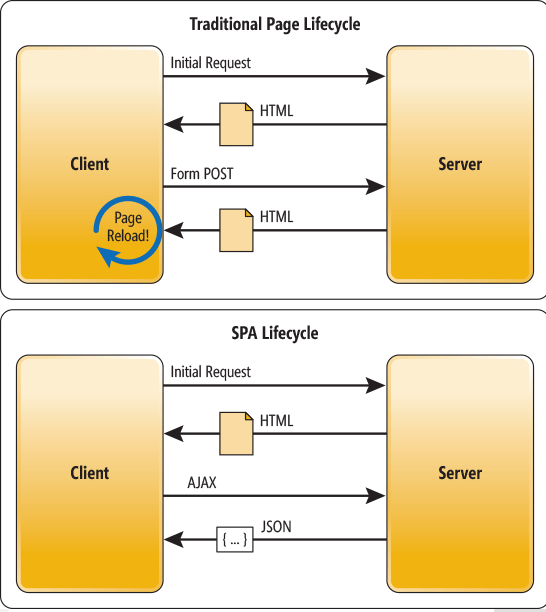
\includegraphics[width=0.8\textwidth]{resources/lifecycle.png}
\caption{Разница в жизненных циклах двух концепций}
\label{a}
\end{figure}

Для ответа на этот вопрос вспомним, что раньше традиционный жизненный цикл страницы работал следующим образом (рис. ~\ref{a}): сервер генерирует много html кода и возвращает его в браузер. Браузер (он же клиент), отображает его. Потом, если мы ходим увидеть изменения на интерфейсе, мы обновляем страницу целиком, а сервер возвращает полностью практически идентичный предыдущему html код с небольшими различиями.

Одностраничные приложения концептуально отличается тем, оно загружают страничку html единожды. С сервера приходит мало html, но много java-script кода, который и генерирует разметку и посылает AJAX запросы с клиента на сервер, на что сервер возвращает данные в формате JSON.

При этом, чтобы узнать, не поменялось ли что-либо на интерфейсе не нужно перезагружать страницу. Может существовать какой-нибудь отдельно взятый блок с java-script, который будет периодически отправлять запросы на сервер, чтобы узнать, не появилось ли новых данных для отображения на клиенте. Если они есть, то возвращаются данные и рендерится маленький кусочек разметки, отвечающий за это, за счет чего сильно экономится трафик. React, Angular и Vue работают именно по принципу Single Page Application, динамически отрисовывая интерфейс приложений с помощью изменения состояния отдельно взятых компонентов.

\section{Кодирование с JSX}

JSX, созданный разработчиками Facebook, фактически является синтаксическим сахаром JavaScript-а.

JSX позволяет нам писать html-элементы в JavaScript и помещать их в DOM без каких-либо createElement() и / или appendChild()методов. Можно не использовать JSX, но JSX облегчает написание приложений React.
\begin{enumerate}
\item
Я--JSX разметка!

\item React.createElement('h1', {}, 'I do not use JSX!');
\end{enumerate}

Оба варианта отобразят одинаковый интерфейс, но код, написанный с JSX выглядит гораздо понятнее и структурированнее. С ним вы можете писать выражения внутри фигурных скобок {}, которое
может быть переменной React, свойством или любым другим допустимым выражением JavaScript.

Html-код должен быть обязательно заключен в один элемент верхнего уровня.
Поэтому, если необходимо вернуть два тега, разработчик должен поместить их в родительский элемент, например div или React.Fragment.
\section{Компонента React}

\subsection{React Props}

Компонента -- это независимая и многократно используемая JSX-разметка. Компоненты служат той же цели, что и функции JavaScript, но работают изолированно и возвращают html через функцию рендеринга. Они принимают произвольные входные данные (так называемые «пропсы») и возвращают React-элементы, описывающие, что мы хотим увидеть на экране.
Компоненты бывают двух типов: компоненты класса и компоненты функции, автор в своей работе автор использовала только первый вариант.

Компоненты могут ссылаться на другие компоненты в возвращённой ими разметке. Это позволяет нам использовать одну и ту же абстракцию — компоненты — на любом уровне нашего приложения. Неважно, разрабатываем ли мы особый заголовок, поле для заполнения или большую страницу: все они представляют собой компоненты в React-приложениях.

Props - это аргументы, передаваемые в компоненты React.
Props передаются компонентам через атрибуты html, используется тот же самый синтаксис. Каждый компонент получает аргумент в виде props-объекта, а также позволяет передавать данные из одного компонента в другой в качестве параметров. React Props доступны только для чтения. Программист получит ошибку, если попытается изменить их значение.

\subsection{React State}
У компонентов React есть встроенный state-объект.
В этом state-объекте хранятся значения свойств, которые принадлежат компоненту.
Когда он изменяется, компонент перерисовывается (перерендеривается).

State-Объект инициализируется в конструкторе (рис. ~\ref{b}):

\begin{figure}[!ht]
\centering
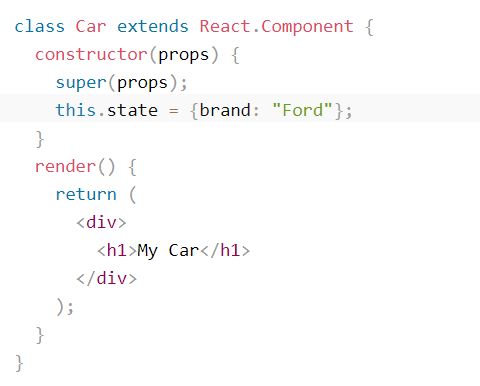
\includegraphics[width=0.8\textwidth]{resources/state.png}
\caption{Инициализация состояния}
\label{b}
\end{figure}

Обратиться к state-объекту можно в любом месте компонента, используя синтаксис this.state.<имя-состояния>. Чтобы изменить значение в объекте состояния, используется this.setState() метод.
Когда значение в state-объекте изменяется, компонент будет повторно перерендериваться.

\subsection{Жизненный цикл в React}

Каждый компонент в React имеет жизненный цикл, который можно отслеживать и манипулировать им на трех основных этапах:

\begin{itemize}
\item Монтирование
\item Обновление
\item Размонтирование
\end{itemize}

Монтирование означает помещение react-элементов в DOM-дерево. В React есть четыре встроенных метода, которые вызываются в следующем порядке при монтировании компонента:

\begin{itemize}
  \item constructor()
  \item getDerivedStateFromProps()
  \item render()
  \item componentDidMount()
\end{itemize}

Метод render() является обязательным и будет вызываться всегда, остальные являются необязательными и будут вызываться, если их работу определить самостоятельно.

Метод constructor() вызывается раньше всего, когда компонент инициализируется, и это же является местом для установки начального состояния и других начальных значений. Данный метод вызывается с props в качестве аргументов, и вы всегда должны начинаться с вызова функции super(props), так как это запускает метод конструктора его родителя и позволяет компоненту наследовать методы от React.Component.

Метод getDerivedStateFromProps() вызывается непосредственно перед отображением элемента(ов) в DOM-дереве. Обычно в данном методе устанавливают значения состояния на основе props-ов. Он принимает state в качестве аргумента и возвращает объект уже с изменённым state.

Метод componentDidMount() вызывается после первоначального рендера компонента.
Здесь можно запустить код, которые требует, чтобы компонент уже был помещен в DOM-дерево.

Следующий этап жизненного цикла — это когда компонент обновляется.
Это происходит всякий раз, когда происходит изменение состояния или props-а компонента.

React имеет пять встроенных методов, которые вызываются в следующем порядке при обновлении компонента:

\begin{itemize}
\item getDerivedStateFromProps()
\item shouldComponentUpdate()
\item render()
\item getSnapshotBeforeUpdate()
\item componentDidUpdate()
\end{itemize}

Метод getDerivedStateFromProps также срабатывает и при обновлении. Это первый метод, который при этой вызывается.
Выполняет те же функции, что и при монтировании.

В методе shouldComponentUpdate() можно вернуть логическое значение, которое указывает, должен ли React продолжать процесс рендеринга или нет.
Значение по умолчанию равняется true.

Логично, что render() вызывается при обновлении компонента, ведь он должен повторно визуализировать html-код в DOM-дереве с новыми изменениями.

В методе getSnapshotBeforeUpdate() есть доступ к props-ам и состоянию до обновления. Это означает, что даже после обновления можно проверить, какие значения были до него.

componentDidUpdate() вызывается после обновления компонента в DOM-дереве. Если пытаться менять состояние в данном методе, то можно получить в результате бесконечный цикл, так как сразу после изменения state произойдет обновление компонента и вновь вызовется componentDidUpdate().

Следующий этап жизненного цикла — это когда компонент удаляется из DOM или размонтируется, как это принято называть в React.

В React есть только один встроенный метод, который вызывается при размонтировании компонента: componentWillUnmount()

\subsection{События в React}

Как и HTML, React может выполнять действия на основе пользовательских событий.
React имеет те же события, что и HTML: щелчок, изменение, наведение мыши и т.д.

События React записываются в синтаксисе camelCase:
onClick вместо onclick.
Обработчики событий React написаны в фигурных скобках:
onClick={show} вместо onClick="show()".
Хорошей практикой является размещение обработчика событий как метод в классе компонента.

Для методов в React ключевое слово "this" должно представлять компонент, которому принадлежит метод.
Вот почему стоит использовать стрелочные функции. С ними this всегда будет иметь контекст объекта, который определил стрелочную функцию.

\subsection{Обработка форм в React}

Как и в HTML, React использует формы, позволяющие пользователям взаимодействовать с веб-страницей.
Обработка форм — это то, как обрабатываются данные, когда они изменяют значение или передаются.
В html данные формы обычно обрабатываются DOM-деревом. В React они обрабатываются компонентами.

Когда данные обрабатываются компонентами, все данные сохраняются в их состоянии.
Тем самым можно контролировать изменение состояния, добавив обработчики событий в onChange атрибут.

Если разработчик не хочет отображать элемент (например button) до тех пор, пока пользователь не сделает какой-либо ввод, он сможет добавить оператор if прямо в метод рендера.
Контролировать действие отправки можно, добавив обработчик события в атрибуте onSubmit.

Очень часто приходится управлять значениями более чем одного поля ввода. Для этого можно добавить name-атрибут к каждому элементу.
Во время инициалзации состояний в конструкторе просто нужно использовать имена полей для ввода.
Чтобы получить доступ к этим полям в методе обработчика используется синтаксис event.target.name и event.target.value.
Обновление состояния обычно делают по принципу: this.setState(\{[event.target.name] : event.target.value\}).

\section{Material-UI для React}

Material UI это библиотека на основе Material Design - вида дизайна, разработанного в 2014 году Google и очень популярного для web и мобильных приложений.
Он вдохновлен физическим миром и его текстурами, включая то, как они отражают свет и отбрасывают тени. Минималистичен, не перегружен деталями.
Данная библиотека позволяет не тратить часы на стилизацию CSS с нуля, а позволяет пользоваться готовыми компонентами. Чтобы начать, нужно иметь знания в React и разобраться в документации на официальном сайте,
где описано, как подключить все зависимости, настроить конфигурацию особого файла muitheme.js. Разработчики хоть и обновляют библиотеку достаточно часто, но их компоненты все равно не исчерпывают все потребности в разработке интерфейса,
но являются отличной базой для собственных.

\section{Стилизация с LESS}

LESS - язык динамических таблиц стилей, а также препроцессор CSS.
LESS расширяет CSS динамическим поведением, таким как переменные, миксины, операции и функции. LESS работает как на стороне клиента (IE 6+, Webkit, Firefox), так и на стороне сервера, с Node.js.

Проще говоря, LESS позволяет писать CSS более умным способом, комбинируя функции, миксины, операции и многое другое. Это означает, что вы пишете более краткую информацию о стилях и можете более легко использовать такие вещи, как цвета и стили.
Препроцессор CSS - это язык сценариев, который является расширением CSS. Он компилируется в обычный синтаксис CSS, а затем CSS читается веб-браузером. Less очень похож на CSS.

Миксины позволяют встраивать все свойства класса в другой класс, включая имя класса в качестве одного из его свойств, и таким образом это работает в своем роде как константа или переменная. Они также могут вести себя как функции и принимать аргументы. CSS не поддерживает миксины, поэтому файлы формата .css содержат так много повторяющегося кода. Миксины обеспечивают более эффективный и чистый код, а также облегчают его изменение.
LESS позволяет использовать операции и функции. Операции позволяют добавлять, вычитать, делить и умножать значения и цвета свойств, которые можно использовать для создания сложных отношений между свойствами, а функции позволяют манипулировать разными значениями прямо внутри LESS файла.

\section{Axios для более приятной работы с запросами}

Axios является одним из самых популярных HTTP-клиентов на основе промисов как для браузеров, так и для Node.js.

По умолчанию он защищает от подделки межсайтовых запросов (XSRF).

// TODO


\chapter{О задаче}

\section{Постановка задачи}

Требуется создать web-приложение, которое упрощает создание и обновление резюме кандидатами и работниками компании Akvelon,
а также решает многие проблемы рекрутеров, оптимизируя их работу и тем самым сокращая время,
проведенное над редактированием документов.

\section{Требуемый функционал}

\begin{enumerate}
\item Возможность создания, копирования, редактирования и архивирования резюме;
\item Наличие базы данных, в которой бы хранились названия компаний, институтов,
проектов, навыков, персональных результатов и сфер ответственности;
\item Автоматическое заполнение перечисленных данных в поля резюме - всплывающие подсказки и поиск по ним;
\item Возможность пополнения этой базы данных как обычными пользователями так и администраторами сайта;
\item Модерация добавленных данных администраторами в один клик;
\item Подобие папок с проектами, на которые можно назначить кандидатов и производить поиск по имени и позиции;
\item Скачивание резюме в формате .docx, стилизованное под стандартное резюме Akvelon;
\item Заполнение общей информации о кандидате с помощью подсказок с логическими выделенными словосочетаниями;
которые превращаются в подобие шаблона при их выборе. Подсказки должны предлагаться в случайном порядке, чтобы повысить уникальность текста в резюме;
\item Пользователь приложения должен иметь возможность указать свою роль на проекте, для которого создается резюме;
Смена этой роли должна вызвать автоматическую пересортировку данных,
чтобы наиболее актуальные для позиции умения находились выше остальных;
\item Сайт нужно создать в стиле Akvelon, придерживаясь дизайна других сервисов данной
компании;
\item Возможность дать другим пользователям права модератора;
\item Блокировка и удаление пользователя;
\item Всплывающие уведомления об ошибках и прочей информации для пользователя;
\item Интерфейс для отслеживания прогресса работы приложения.
\end{enumerate}

\section{Используемые программные средства}

Исходя из того, что требуется написать клиентскую часть приложения, для разработки были выбраны следующие программные средства:

\begin{itemize}
\item VSCode для разработки и отладки приложения;
\item JavaScript в качестве основного языка программирования;
\item GitLab для управления репозиторием кода для Git;
\item MobX для управления состоянием приложения;
\item Axios для взаимодействия с API;
\item React.js для создания интерфейса;
\item Material UI для создания единого стиля компонентов;
\item LESS для корректировок стиля Matreial и для создания собственного;
\item Jest и Enzyme для написания unit-тестов.
\end{itemize}

\chapter{Решение задачи}

\section{Создание базовой архитектуры}
В компании мне предоставили готовый шаблон со структурой, где уже подключен Webpack, настроено несколько правил ESLint для поддержания кода чистым и более приятным глазу.
Для начала разработки была реализована следующая структура проекта в директории src:

\medskip

\renewcommand*\DTstyle{\ttfamily\textcolor{black}}
\dirtree{%
.1 /.
.2 components.
.2 containers.
.2 services.
.3 action.notify.
.3 toast.notify.
.3 stores.
.3 request.services.
.3 validator.
.2 app.js.
.2 app.less.
.2 constants.js.
.2 index.html.
.2 muitheme.js.
.2 router.js.
.2 variables.less.
}

\begin{itemize}
\item Папка components предназначена для react-компонентов для многоразового использования, непривязанных к какому-либо контексту, желательно максимально абстрактных.
\item Containers - каталог для логически разделенных папок, содержащих в себе компоненты конкретных страниц.
\item Services - папка для сервисов, которые отвечают за реализацию кода, независимого от внешнего окружения. В данном приложении понадобились сервисы для логики полос прогрузки данных, появления уведомлений, взаимодействия с API, валидации, и действий с observable-состаяниями MobX-а.
\item index.html - точка входа приложения, в нем описываются подключения стилей и скрипта для рендера.
\item index.js указывает, в какую область html документа будет проецироваться DOM-дерево и рендерит app.js.
\item app.js содержит компоненты-провайдеры, отвечающие за авторизацию, инициализацию MobX stores, стилей-muitheme и перенаправления на страницы.
\item app.less - в этом файле написаны общие стили, которые используются практически во всех компонентах.
\item constants.js - переменные, которые используются в разных местах программы по типу предложений, коэффициентов, регулярных выражений.
\item muitheme.js - файл, позволяющий задать конфигурации Material UI стилей.
\item router.js - компонент-маршрутизатор, определяет какой обработчик надо вызвать для конкретного маршрута.
\item variables.less - содержит палитру именных основных цветов сайта. Файл служит для удобства, чтобы было проще ориентироваться на название переменной, а не на HEX или RGB коды.
\end{itemize}

\section{Создание сервиса запросов, авторизация}

Первым делом предстояло как-то идентифицировать пользователей, для чего я создала первый сервис в папке services - request.service со следующей структурой:
\medskip
\dirtree{%
.1 request.service.
.2 api.
.3 auth.js.
.2 index.js.
}
\medskip

index.js содержит логику неявной авторизации, а также функцию sendRequest, отвечающую за то, чтобы во все заголовки запросов подкладывался валидный token.

auth.js -- один из классов с асинхронными функциями, которые формируют axios-конфигурацию для отправки запроса на сервер.
Для авторизации понадобились следующие функции:

\begin{enumerate}
\item signUp -- выполняет POST-запрос, в котором отправляются данные для инициализации нового пользователя;
\item signIn -- POST-запрос, который принимает логин и пароль, а в ответ мы получаем информацию о пользователе, его refresh и access token;
\item refresh -- POST-запрос, в котором отправляется refresh-token, чтобы обратно получить access-token. Refresh хранится в locale storage -- постоянном хранилище данных --
и его действие истекает через месяц полного бездействия аккаунта, в то время как access-token "живет" пол часа и обновляется каждый раз, когда пользователь перезагружает страницу, при условии, что refresh еще актуален;
Все это позволяет не хранить в целях безопасности access-token в локальном хранилище. И даже если злоумышленник вдруг перехватит access-token, то у него будет лишь пол часа. Также эта идея позволяет пользователю сэкономить время на вбивание данных для входа. Страницу со входом можно будет наблюдать в случае, если человек выйдет из аккаунта сам или если пройдет месяц и его refresh-token станет невалидным;
\item getPermissions -- GET-запрос, который возвращает информацию о правах, чтобы различать админа от рядового пользователя.
\end{enumerate}

Теперь, когда запросы описаны, я написала компонент-обертку над app.js, в которой происходит логика неявной авторизации, если пользователь перезагружает страницу.

В классе AuthorizaionProvider в конструкторе задается начальное состояние компонента -- isAuthorized, равное false. Пока оно false, на интерфейсе отображается только белый фон с полосой загрузки. При каждом первоначальном рендеринге (монтировании) этого компонента
вызовется функция silentAuthorization, обернутая в try/catch. Она выполняет следующие действия:

\begin{enumerate}
\item Из локального хранилища достается refresh-token;
\item Этот refresh отправляется на сервер, ожидая получить новый access-token;
\item Если с момента входа в аккаунт прошел месяц и refresh истек, то возвращается ошибка, срабатывает catch и пользователя перенаправляет на страницу входа, чтобы он зашел вновь;
\item Если нет, то внутри программного кода сохраняется access-token, а в локальное хранилище записывается новый продленный refresh;
\item Определяются права пользователя;
\item isAuthorized становится true и пользователю доступен интерфейс приложения.

\end{enumerate}

\section{Регистрация, валидация и вход на сервис}

Клиент поставил условие -- страницы, связанные с авторизацией должны быть выполнены в таком же стиле, что и сайт компании для
оценки рабочего времени, написанный на Vue.js. Но должна быть возможность входа с любой почтой, а не с доменным именем.

\begin{figure}[!ht]
\centering

\includegraphics[width=0.8\textwidth]{resources/ets.png}
\caption{Страница входа на ets.akvelon.com}
\label{fig:1}
\end{figure}

По итогу было сделано максимально возможно похоже, но с помощью React, LESS и Material-UI компонентов (рис. ~\ref{2}):

\begin{figure}[!ht]
\centering

\includegraphics[width=0.8\textwidth]{resources/signin.png}
\caption{Страница входа на hrcv.inyar.ru}
\label{2}
\end{figure}

Следующий шаг — сделать валидацию на странице регистрации. Для этого я создала еще один сервис со следующей архитектурой.
\medskip
\dirtree{%
.1 validator.
.2 isValidPassword.
.2 isEmail.js.
.2 isNotEmpty.js.
.2 isValidLength.js.
.2 isValidName.js.
}
\medskip

В результате работы этих функций возвращается булевый результат и сообщение об ошибке, если он false.
Если ошибки могут быть разного типа для одного поля ввода, то сначала покажется одна, а уже при ее исправлении -- следующая.
\medskip

\begin{itemize}
\item isNotEmpty проверяют строку на пустоту. С помощью функции JavaScript trim() удаляются пробелы, а длина того, что осталось сравнивается с нулем.
\item isValidLength проверяет строку на соответствие минимальной и максимальной длине строки, переданных в функцию.
\item isValidPassword и isValidName проверяют строку на соответствие регулярному выражению из файла constants, вызывает внутри isNotEmpty и isValidLength.
\item isEmail валидирует строку на корректное написание e-mail, условия успешной проверки хранятся в constants.
\end{itemize}

Также в целях интереса и знакомства с технологией добавлена ReCAPTCHA — система, разработанная в университете Карнеги-Меллон для защиты веб-сайтов от интернет-ботов.

В SignUp react-компоненте заведены состояния для каждого условия успешной регистрации на сайте. Пока все условия не пройдут проверку, кнопка login будет заблокирована,
а рядом с полями, в которых допущена ошибка будут отображаться наглядные красные сообщения.

\begin{figure}[!ht]
\centering
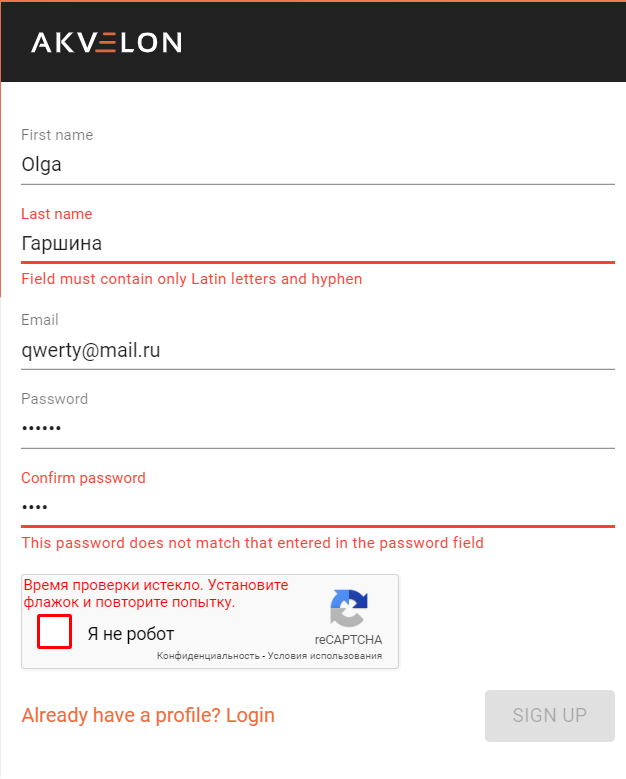
\includegraphics[width=0.7\textwidth]{resources/signup.png}
\caption{Страница входа на ets.akvelon.com}
\label{fig:1}
\end{figure}

\section{Сервис уведомлений пользователя, отслеживание прогресса загрузки}

На данном этапе разработки понадобилось оповещать пользователя об ошибках со стороны сервера и другой полезной информации.
Для этого я создала сервис toast.notify и ToastTrigger компонент.

В этом компоненте инициализируются состояния, отвечающие за отслеживание того, отображается плашка с оповещениями или нет, за текст сообщения и за тип уведомления.
При монтировании ToastTrigger как бы говорит toast.notify сервису, что если в коде в каком-нибудь месте вызовется функция-уведомитель, в параметрах которой будут переданы сообщение и тип уведомления -- состояние
компонента должно поменяться соответственно. На рисунке ~\ref{4} отражен вызов функции в месте кода, где сервер вернул ошибку добавления новой категории.

\begin{figure}[!ht]
\centering
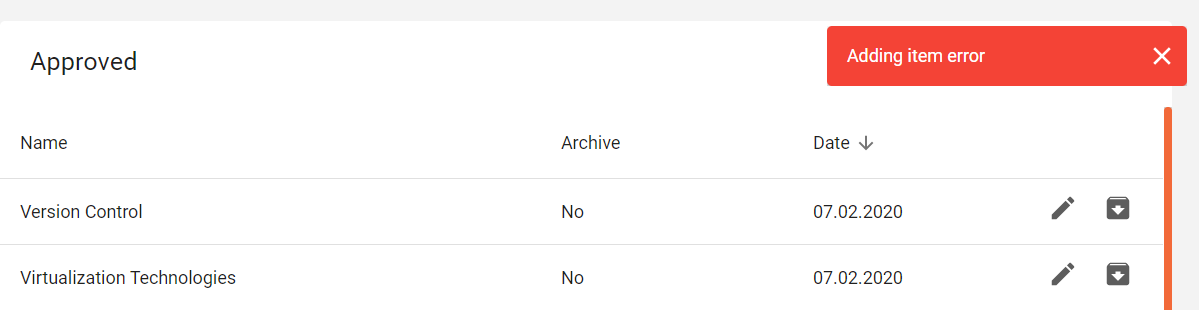
\includegraphics[width=0.9\textwidth]{resources/toasterror.png}
\caption{Пример уведомления об ошибке}
\label{4}
\end{figure}

Я поделила оповещения на 4 типа: предупреждение, ошибка, информация и успех. С помощью
LESS очень удобно переопределять стиль плашки в зависимости от параметров, переданных в
функцию. Вот, например, плашка с информацией, которая вызывается при попытке сохранения резюме, если пользователь
забыл ввести обязательную информацию (рис. ~\ref{5}).

\begin{figure}[!ht]
\centering
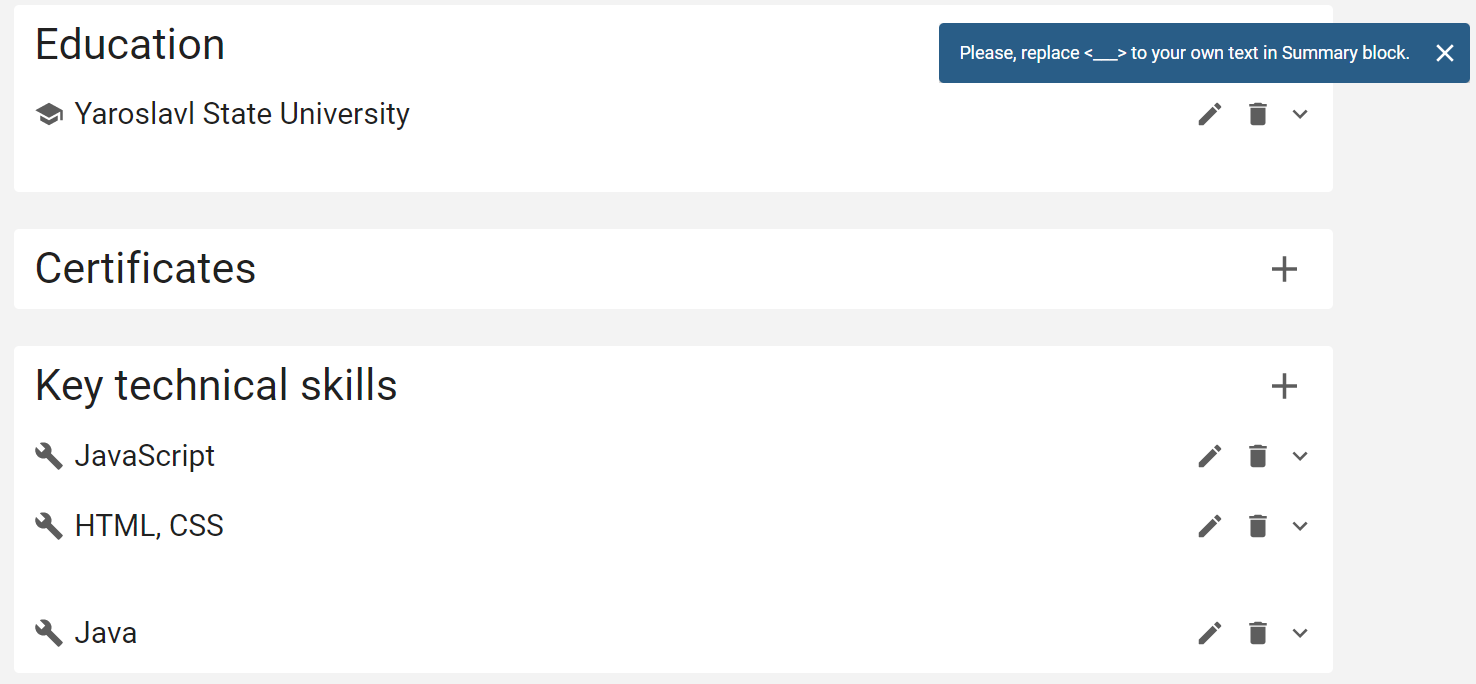
\includegraphics[width=0.9\textwidth]{resources/toast.png}
\caption{Пример информационного уведомления}
\label{5}
\end{figure}

Что касается сервиса, показывающего прогресс, то он сделан похоже, за исключением того, что action.notify хранит массив
из подписок на события, которые должны вызывать полосы загрузки. Таким образом на странице может отображаться сразу несколько полос прогресса получения данных в разных местах. Достаточно обернуть их
компонентом LoaderTrigger, передав имя события, на которое подпишется сервис.

Данный пример иллюстрирует отображение полос прогресса, пока с сервера подгружаются коллекции компаний и обрабатывается запрос на перенос компании из списка предложенных в список одобренных (рис. ~\ref{6}).
На самом деле это делается мгновенно и полоса прогрузки является больше дружественным интерфейсом для пользователей с медленным интернетом. Для отображения прогресса достаточно вызвать две функции: перед началом асинхронного запроса на сервер, передав параметр "start" и после его окончания, передав "finish".

\begin{figure}[!ht]
\centering
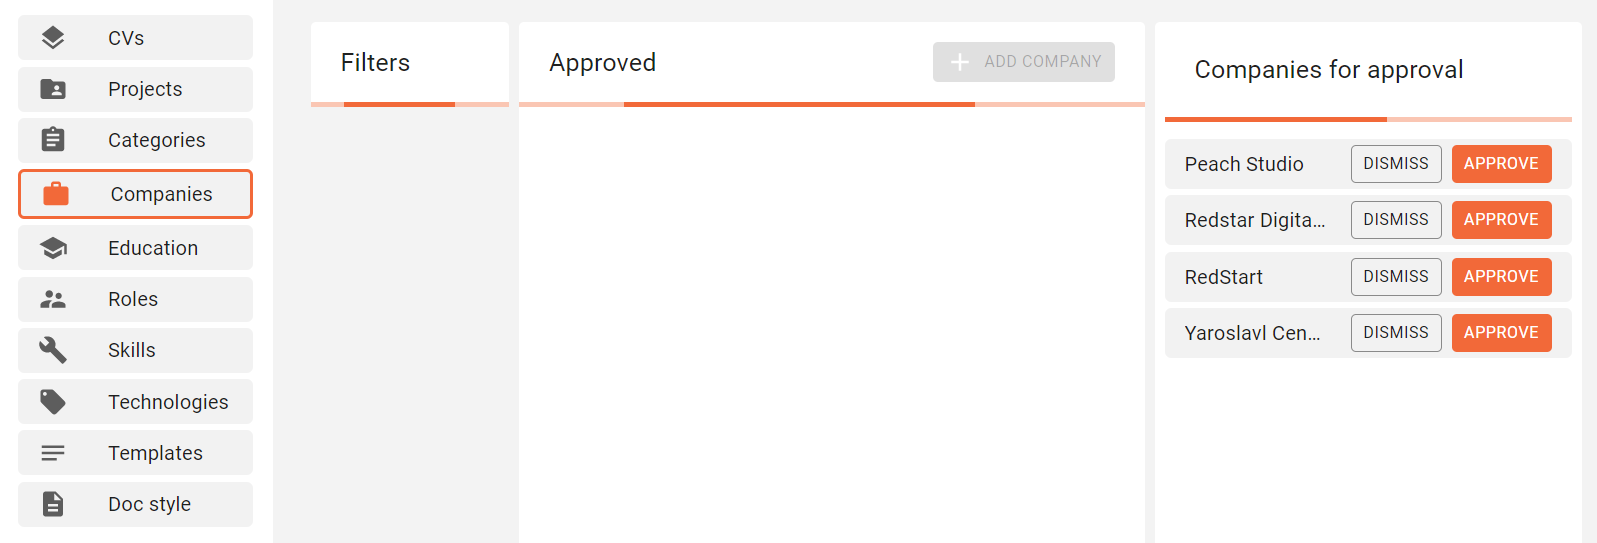
\includegraphics[width=0.9\textwidth]{resources/progress.png}
\caption{Интерфейс полос загрузки}
\label{6}
\end{figure}

\section{Страница создания резюме взглядом пользователя}
Создание резюме проходит в несколько этапов и создается для отправки клиенту Akvelon на определенный проект.
Для начала выбирается роль, в зависимости от которой будут подсказываться автоматические предложения для заполнения и сортироваться технологии, которые знает кандидат. Это значит, что тестировщику, например, будет подсказываться текст,
связанный с написанием UNIT-тестов, а специалисту DevOps - с настройкой CI/CD процессов.

Клиент пожелал, чтобы данные подсказки предлагались в случайном порядке -- это сделает резюме более уникальным, если его будет заполнять не специально обученный рекрутер, а кандидат на позицию.
Далее заполняется поле Summary - краткая выжимка об умениях и качествах работника. В данном поле при нажатии на пункт меню конкретные словосочетания превращаются в шаблоны, выделенные жирным -- такое поведение также попросил заказчик.

Как можно заметить, все это (рис. ~\ref{7}) не похоже на типичное поведение обычного компонента текстового поля из Material UI. Все потому, что данный интерфейс -- это
замаскированный под material design с помощью LESS фреймворк Draft.js -- текстовый редактор, переделанный под мои нужды. Было потрачено немало времени, чтобы разобраться в работе библиотеки,
убрать лишние детали и добавить нужные.

\begin{figure}[!ht]
\centering

\includegraphics[width=1\textwidth]{resources/summary.png}
\caption{Интерфейс заполнения поля Summary}
\label{7}
\end{figure}

Поле роль — созданный мною компонент. Изначально, в Material UI не было достойного решения для выбора пункта из списка, с полем для поиска по нему.
Мне предлагали только сторонние библиотеки, которые имели в себе много лишних зависимостей и строк кода, котор неприятно читать и сложно в них разбираться.
После чего наступил переломный момент и я решила написать свой компонент с тем поведением, который идеально мне подошел. Несмотря на то, что создание простого казалось бы списка со встроенным поискам выглядело тривиальной задачей,
в процессе написания я столкнулась со многими подводными камнями, связанными с обработкой событий в React. Я искала ответы в интернет сообществах по программированию,
но встречала только некрасивые решения.

В итоге мне удалось сделать компонент (рис. ~\ref{8}), отвечающий желаемому функционалу и хранящий в состоянии не строку, а целый объект, что
не тратит ресурсы программы на дополнительные преобразования перед отправкой запроса на сервер.

\begin{figure}[!ht]
\centering
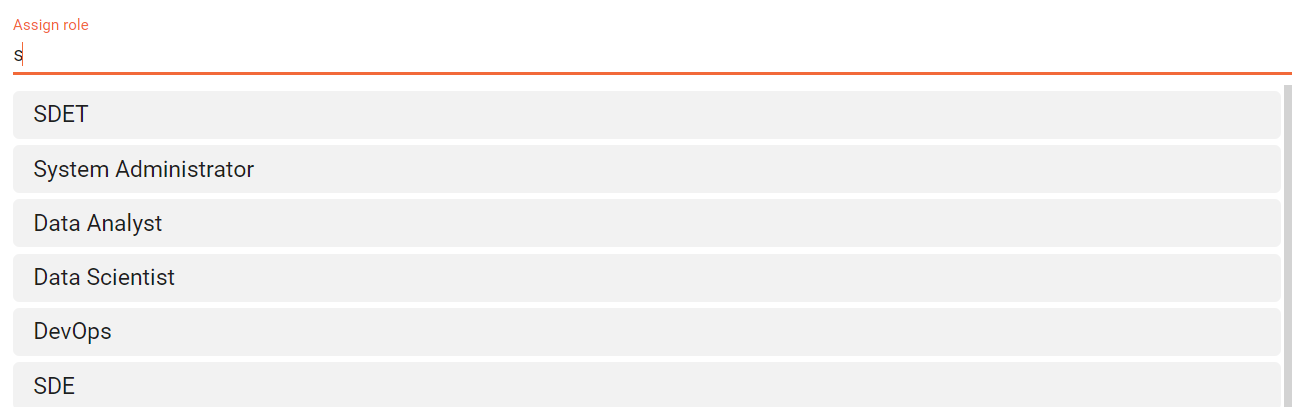
\includegraphics[width=0.8\textwidth]{resources/role.png}
\caption{Компонент для выбора из списка с поиском}
\label{8}
\end{figure}

После кандидат заполняет информацию об опыте работы в компаниях в блоке professional expirience. Я вдохновлялась дизайном заполнения информации на сайте linkedin при разработке данного блока (рис. ~\ref{9}).
На его примере я хочу показать функционал подсказок для автозаполнения и принцип пополнения базы данных.
\begin{figure}[!ht]
\centering
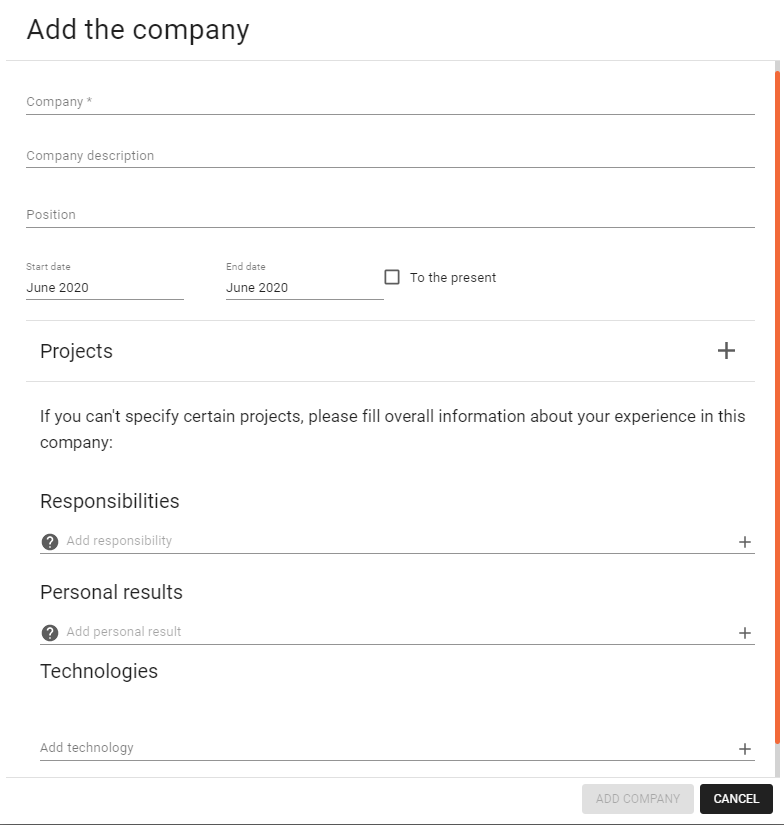
\includegraphics[width=1\textwidth]{resources/companycard.png}
\caption{Диалоговое окно добавления компании}
\label{9}
\end{figure}

Как только пользователь начинает набирать текст в поле Company, под ним раскрывается список тех компаний для заполнения, которые включают в себя набранное буквосочетание.
Если база не включает в себя название компании, которое хочет вбить кандидат, то после нажатия кнокпи "Add" она
отправляется на рассмотрение админами в часть интерфейса, скрытого от обычного пользователя.

Далее идут обычные текстовые поля для заполнения краткой сводки о компании и о занимаемой позиции в ней.

После кандидату необходимо указать время работы в компании. При нажатии на поля start date/end date поочередно открывается интерфейс для выбора года и месяца (рис. ~\ref{10}).
В случае, если кандидат все еще является сотрудником описываемой компании, он может нажать галочку рядом с "To the present", тем самым автоматически скроется возможность выбора даты окончания работы.

\begin{figure}[!ht]
\centering

\includegraphics[width=1\textwidth]{resources/dates.png}
\caption{Интерфейс выбора даты}
\label{10}
\end{figure}

Потом подразумевается заполнение информации о проектах. Если кандидат не может выделить каких-то конкретных, то требуется заполнить общую информацию. Предлагается внести данные о персональных результатах, выполненных задачах и используемых технологиях.
Некоторые люди сталкиваются с проблемой того, что они не могут сразу быстро вспомнить все свои достижения.
Для этого я добавила возможность раскрыть по кнопке со знаком вопроса меню с подсказками шаблонных фраз, которые как и в поле Summary относятся к выбранной в начале роли. Если кандидат оставил место для шаблона незаполненным -- это валидируется.
Описанный выше функционал можно наблюдать на рисунке ~\ref{11}.

\begin{figure}[!ht]
\centering
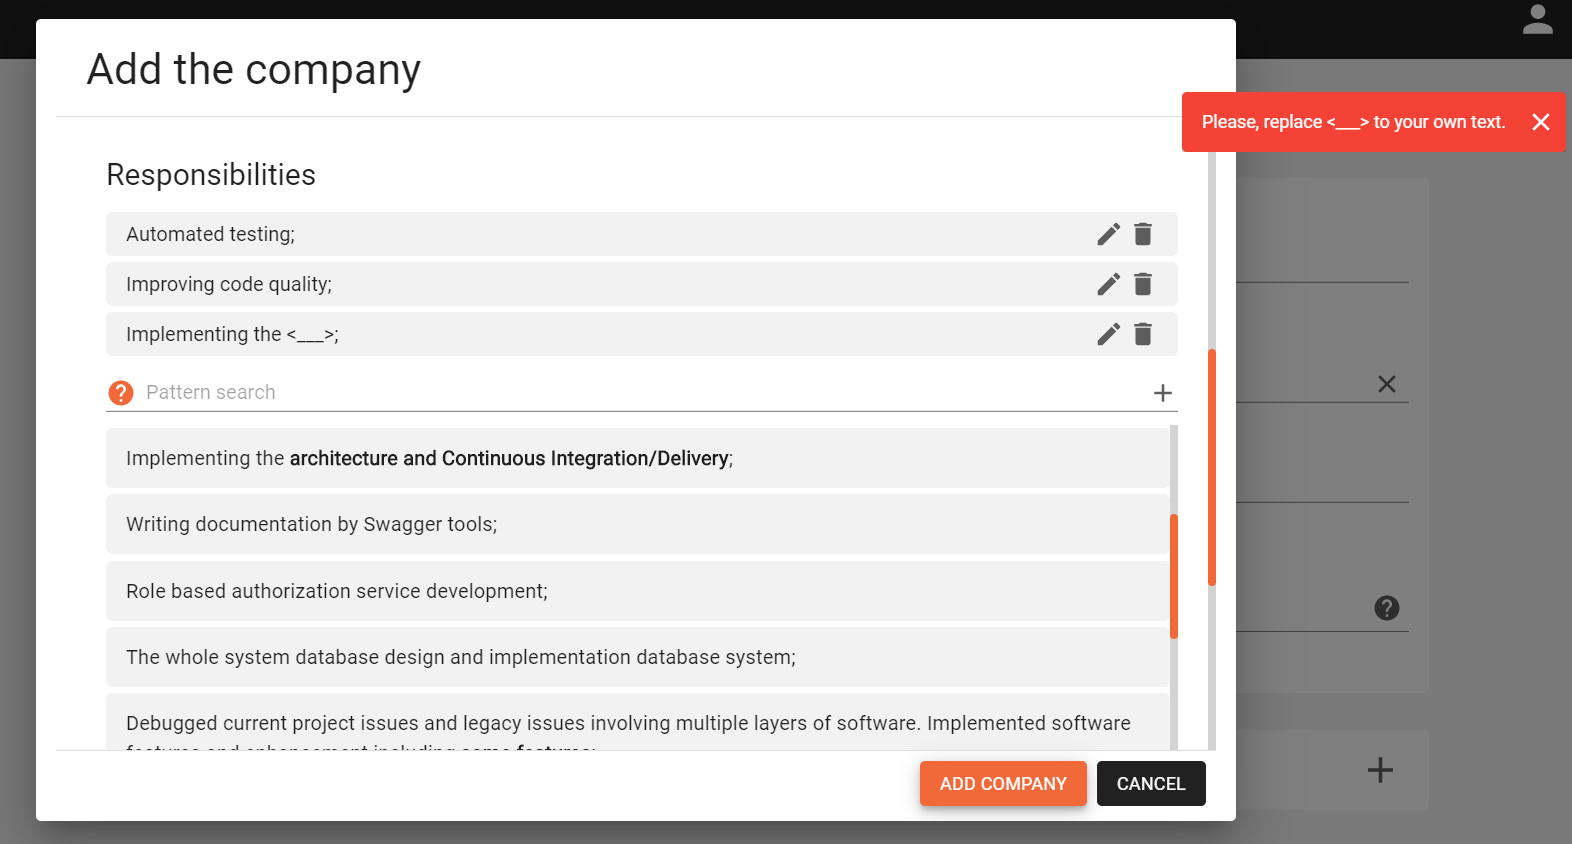
\includegraphics[width=1\textwidth]{resources/responsibility.png}
\caption{Интерфейс заполнения информацией поля responsibility и её валидация}
\label{11}
\end{figure}

Заполнение блока заканчивается указанием используемых в компании технологий, которые автозаполняются и попадают в базу данных на рассмотрение админами.
Так как технологии являются коллекцией с самой большой базой, их модерация достойна отдельного внимания. Чтобы глаз рекрутера мог зацепиться за потенциальное некорректное слово, я
сделала цветовой акцент на интерфейсе. Таким образом, одобренные технологии окрашены в оранжевый, а остальные в серый (рис. ~\ref{12}). Чтобы пользователь не засорял базу альтернативными названиями технологий было решено привязывать к ним список синонимов. Так, введя в поле JS и нажав ввод,
кандидат получит корректное названия языка на выходе -- JavaScript.

\begin{figure}[!ht]
	\centering
	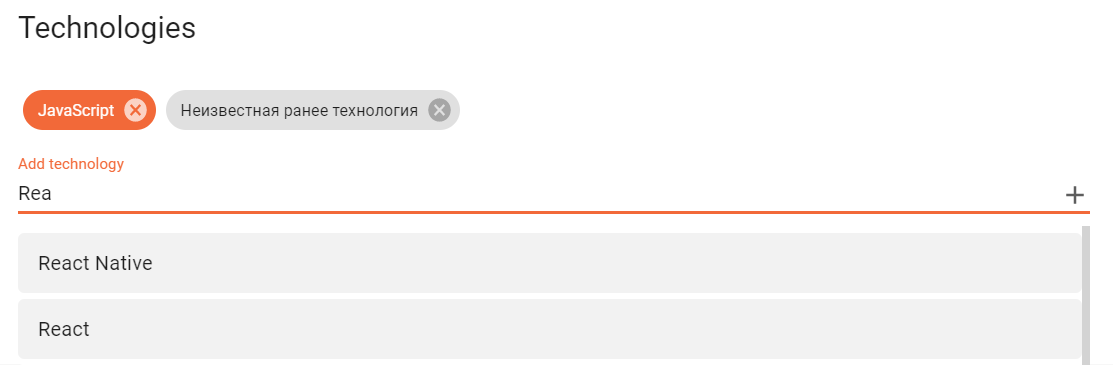
\includegraphics[width=1\textwidth]{resources/technologies.png}
	\caption{Заполнение инфо-блока технологиями}
	\label{12}
\end{figure}

Если же проекты к заполнению все же есть, то по нажатию на плюс всплывает еще одно диалоговое окно, где нужно
указать название проекта, его описание и те же пункты, что и в блоке добавления после выбора времени работы на позиции.

Всё доступно для редактирования и полного удаления, все информационные списки можно сворачивать и разворачивать. Чтобы ненужная на момент заполнения информация не мешала на фоне в развернутом состоянии, в режиме редактирования CV находится
только один логический блок.

Преимущество данного UX-решения особенно хорошо наблюдается в режиме просмотра резюме. В нем можно развернуть всю структуру документа для полноты восприятия, страница приложения станет действительно длинной (рис. ~\ref{13}), особенно если речь идет об опыте работа программиста-сеньора.
Также в данном режиме полностью отсутствуют отвлекающие кнопки для какого-либо взаимодействия, он отлично подходит для того, чтобы рекрутер мог просто поделиться ссылкой на страницу с голой информацией о резюме.

Блоки education, certificates и key technical skills по своей структуре похожи на блок professional expirience, а вот technical summary хочется уделить особое внимание.
В нем автоматически сгенерирован и категоризирован список всех технологий, который пользователь затрагивал, заполняя резюме. Блок меняет свой вид при изменении роли, потому что у программиста с большим стеком он
громаден, а клиент хочет сэкономить свое время и увидеть приоритетную для него информацию в первых же строках. Если технологию указывают в резюме на различных проектах и различных компаниях, написанный мною алгоритм валадирует хранение в данном списке только уникальных наименований технологий.


Также это то место, где кандидат может вбить изученные им вне работы технологии. Иногда бывало, что это тоже играло роль, когда клиенты Akvelon-а выбирали, на какой стек поставить работника на проекте.

Технологии, категории которых не определены, всегда попадают в Others по регламенту стандартного Akvelon-резюме. Список категорий у каждой роли свой и фиксирован, поэтому если кандидат не знает ни одной технологии из категории, ее строка остается пустой (рис. ~\ref{13}).
\begin{figure}[!ht]
\centering
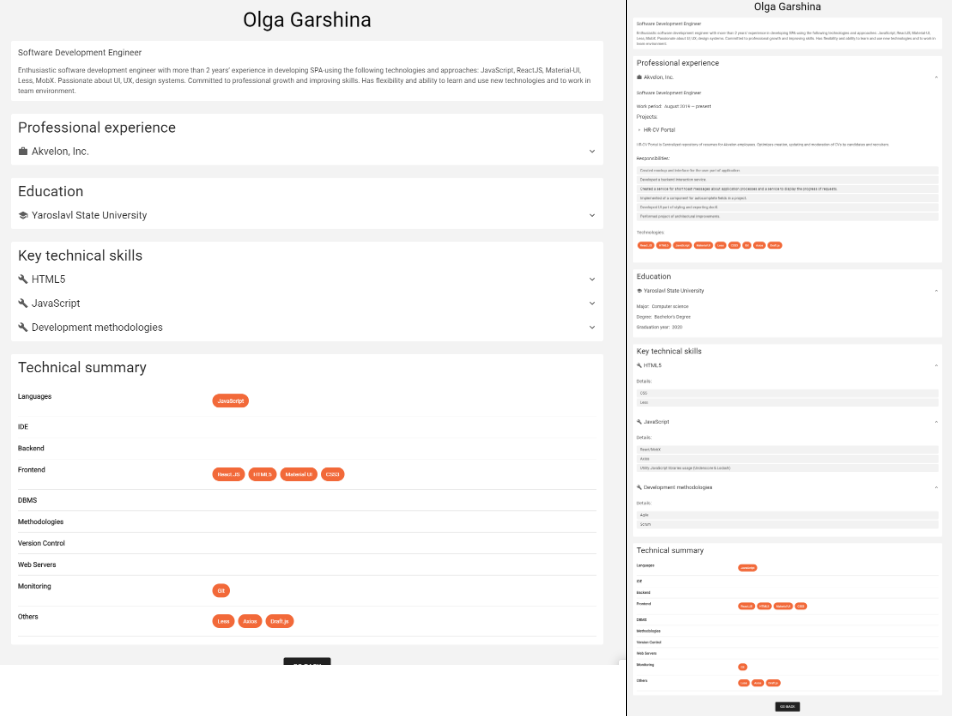
\includegraphics[width=1\textwidth]{resources/expand.png}
\caption{Слева отображен режим просмотра с примером со свернутыми инфо-блоками, справа с развернутыми}
\label{13}
\end{figure}
\section{Таблица всех резюме взглядом пользователя}

Для удобства поиска резюме и фильтрации была реализована идея с таблицей (рис. ~\ref{14}). Фильтрацию можно воспроизводить по имени, роли, позиции,
проекту, по дате и по типу резюме исходя из того, скрыт он от глаз или нет. В зависимости от нужд пользователя, количество строк в таблице можно менять от 5 до 50 на странице.
Нажимая на кнопку с троеточием кандидат может заархивировать (спрятать) резюме, копировать, перейти в режим редактирования или просмотра, а также экспортировать
стилизованный документ в формате .docx. Пользователь может знать информацию о проекте, к которому привязано его резюме, но не может изменить ее, так как эта привилегия рекрутеров, которые подразумеваются
администраторами сайта.

Для экспорта файла была использована библиотека FileSaver.js. Она является решением для сохранения файлов на стороне клиента и идеально подходит для веб-приложений, которым необходимо создавать файлы, или для сохранения конфиденциальной информации, которую не следует отправлять на внешний сервер.


\begin{figure}[!ht]
\centering
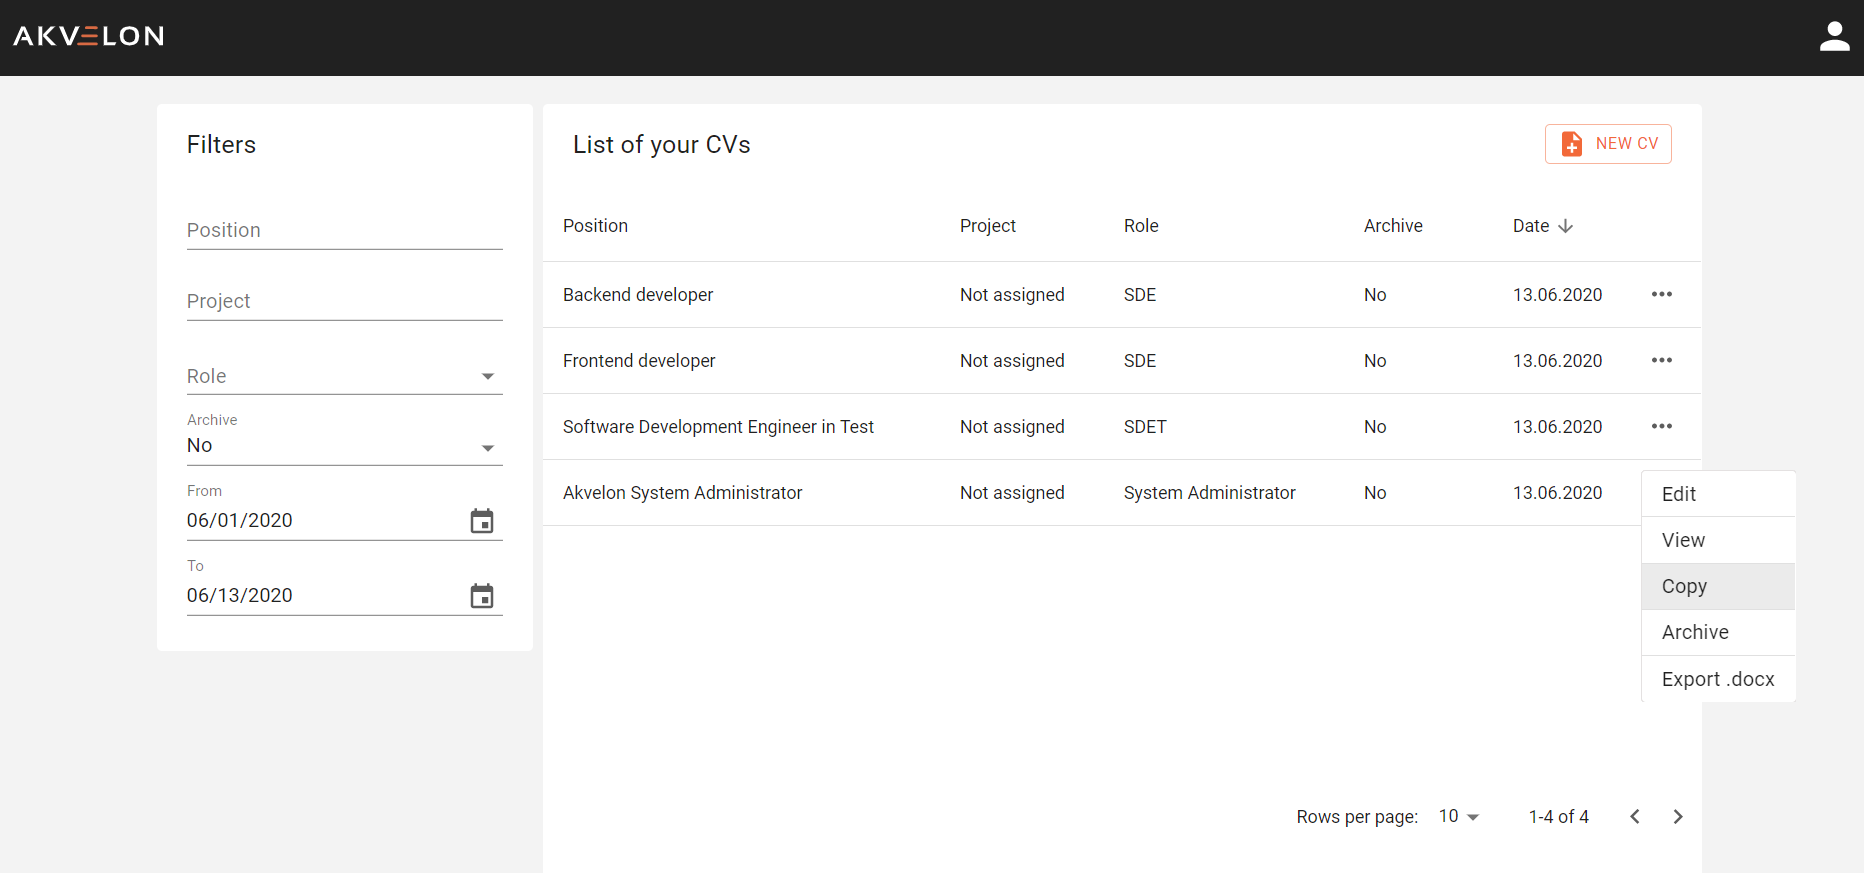
\includegraphics[width=1\textwidth]{resources/cvlistuser.png}
\caption{Таблица со списком пользовательских резюме}
\label{14}
\end{figure}

\section{Интерфейс резюме взглядом администратора}

Приложение со стороны администратора имеет весь набор функционала, доступный обычному пользователю. Но прав и возможностей для модерирования гораздо больше.

Что касается создания резюме, то администратор может создать его для себя (если он по совместительству кандидат) и для другого пользователя (рис. ~\ref{15}). В планах расширить функционал в сторону создания резюме для гостей (незарегистрированных пользователей), чтобы
они смогли заполнить его по временной ссылке. В случае желания зарегистрировать аккаунт, CV бы прикрепилось к пользователю.

\begin{figure}[!ht]
\centering
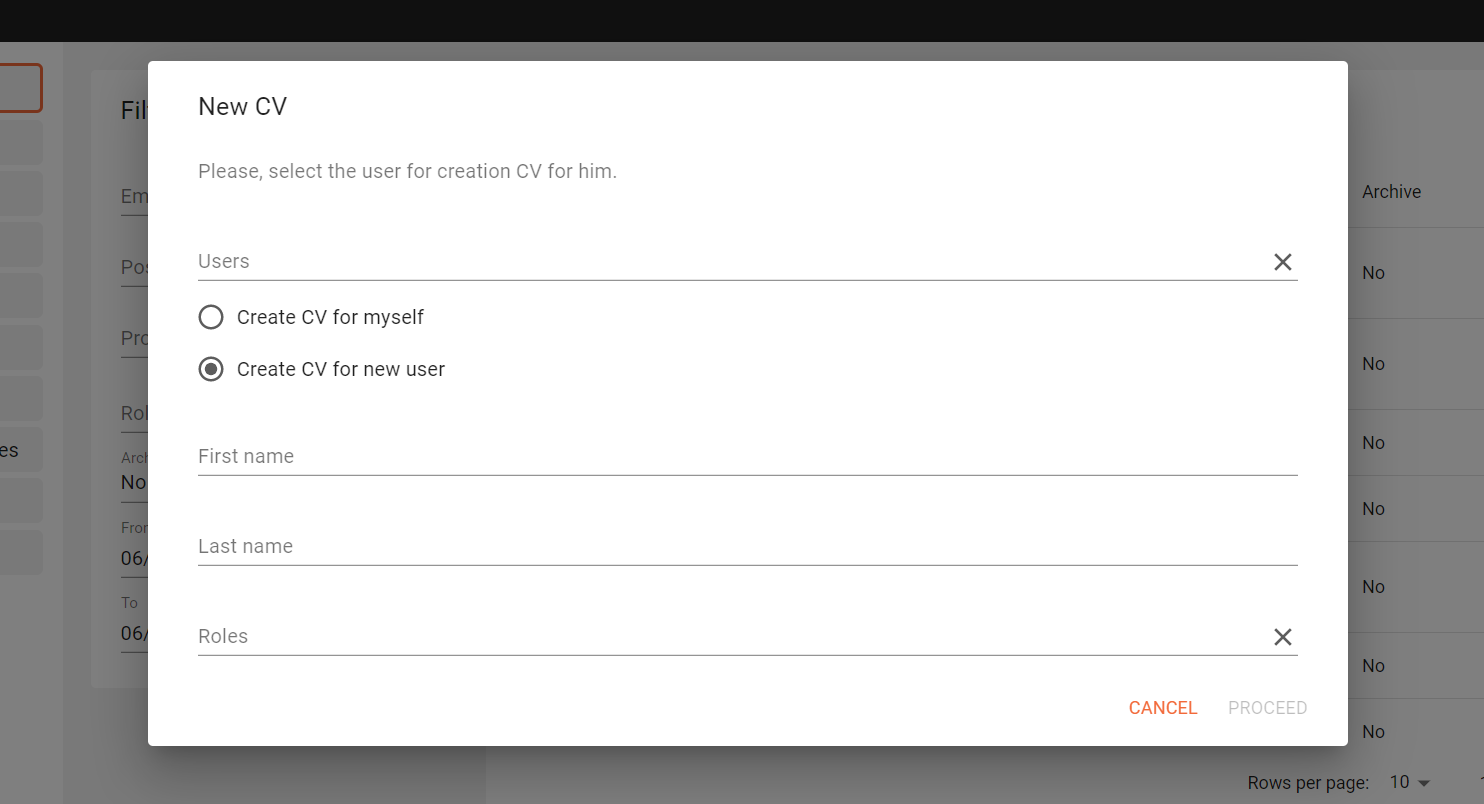
\includegraphics[width=1\textwidth]{resources/newcvdialog.png}
\caption{Диалог перед созданием резюме на интерфейсе администратора}
\label{15}
\end{figure}


На странице создания резюме рекрутер может назначать его на определенный проект. На работе они специально создают папки на компьютере, чтобы хранить резюме для разных проектов отдельно. С HRCV не нужно создавать каталоги под каждый признак, а достаточно произвести фильтрацию на главной странице.

В верхнем правом углу находится вкладка с настройками. По нажатию администратор перейдет к списку всех пользователей ресурса. Он может произвести поиск по имени и выбрав необходимое кликнуть по пункту меню и перейти на профиль данного человека.

В профиле (рис. ~\ref{16}) рекрутер может получить дать права администратора или отнять их, может заблокировать пользователя и тогда он не зайдет в свой аккаунт.
Также присутствует кнопка удаления аккаунта. При нажатии на нее конечно же несколько раз уточняется, правда ли админ хочет это сделать, поскольку это необратимый процесс, который повлечет удаление из базы все резюме, привязанных к данному профилю.


\begin{figure}[!ht]
\centering
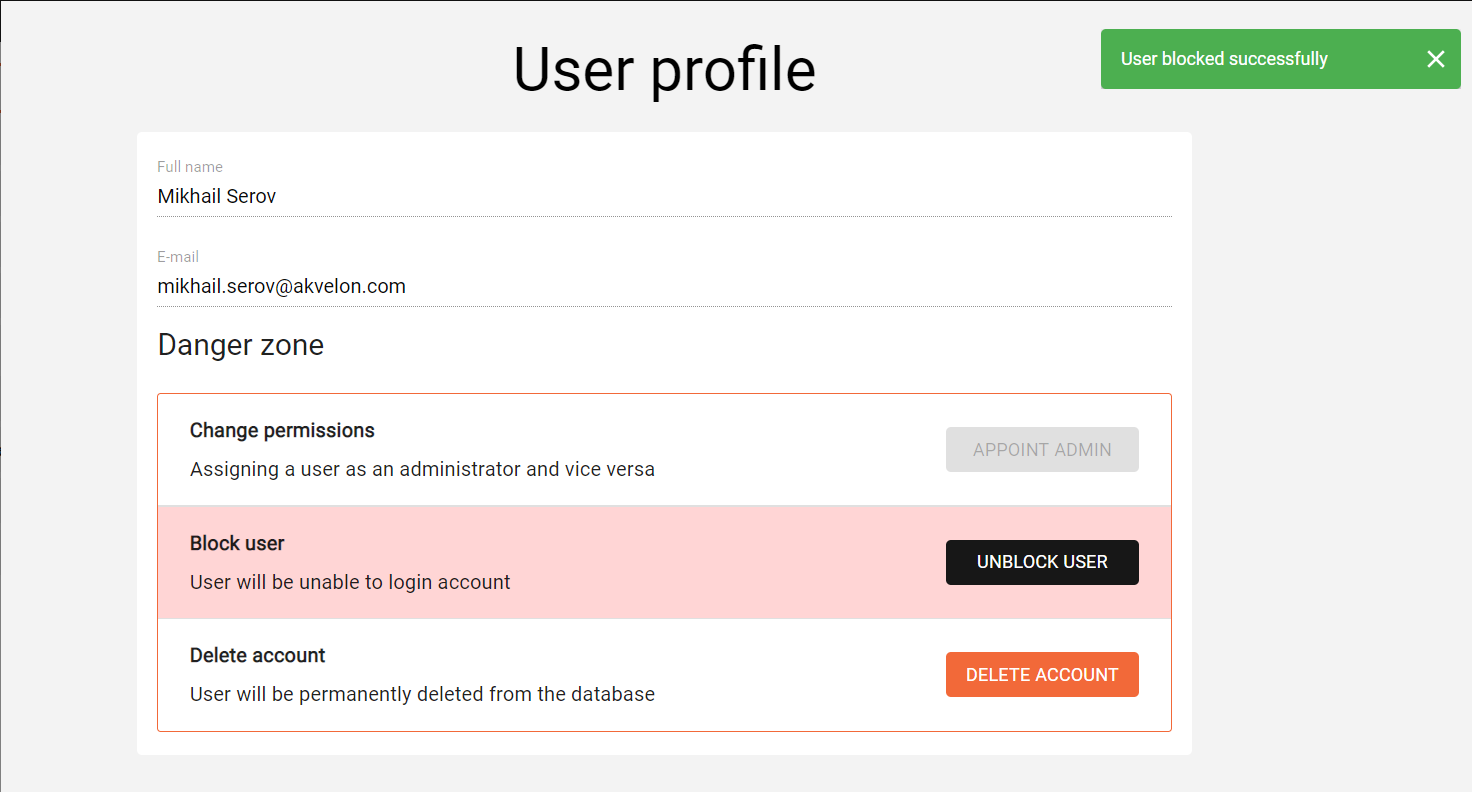
\includegraphics[width=1\textwidth]{resources/dangerzone.png}
\caption{Пример блокировки пользователя}
\label{16}
\end{figure}

Самым главным отличием админского интерфейса от пользовательского является наличие меню слева страницы, в которых модерируются коллекции базы данных и изменяется конфигурация стилей для экспортируемого .docx документа. Во всех коллекциях можно производить фильтрацию, добавлять новые экземпляры, редактировать их и отправлять в архив.

На данный момент разработки существуют списки компаний, категорий технологий, самих технологий, названий учебных учреждений, ролей, навыков и шаблонных строк для автозаполнения. Компании, технологии и учебные заведения отличаются тем, что их может как одобрить (после чего элемент отправляется в базу данных и в таблицу), так и отклонить администратор в
специальном меню на странице их коллекции (рис. ~\ref{17}).

\begin{figure}[!ht]
\centering
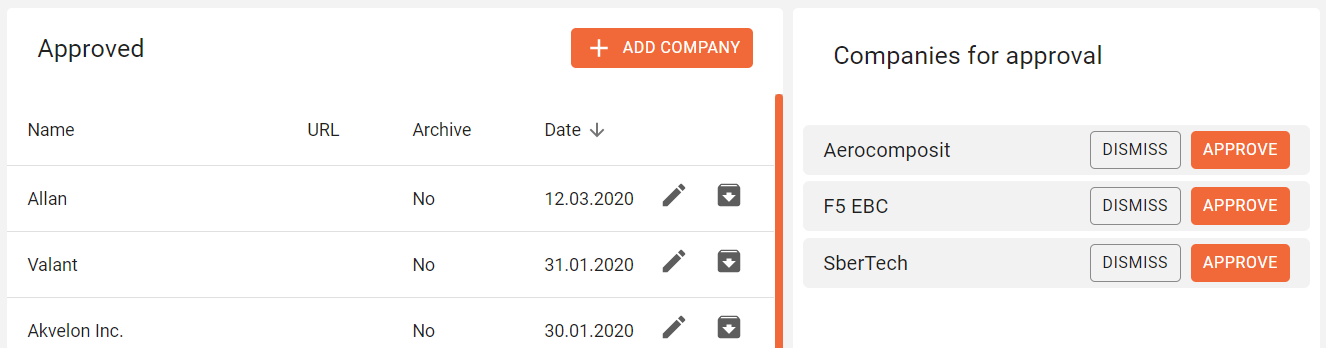
\includegraphics[width=1\textwidth]{resources/companies.png}
\caption{Меню для утверждения или отклонения новых компаний}
\label{17}
\end{figure}
После списка CV идет таблица, отображающая коллекцию проектов. Это то самое подобие папок с проектами, которые просил клиент. Сначала нужно отправить POST-запрос на добавление в коллекцию
путем нажатия на кнопку "Add project" и прописав название. После чего можно назначить резюме на проекты их список появится в разделе проектов при нажатии на кнопку редактирования (рис. ~\ref{18}).

Далее идет список категорий, который имеет уже описанный выше функционал, впрочем, как и коллекция учебных учреждений.

После следует список компаний, к описанию конкретной компании опционально прилагается ссылка на ее сайт.

\begin{figure}[!ht]
\centering
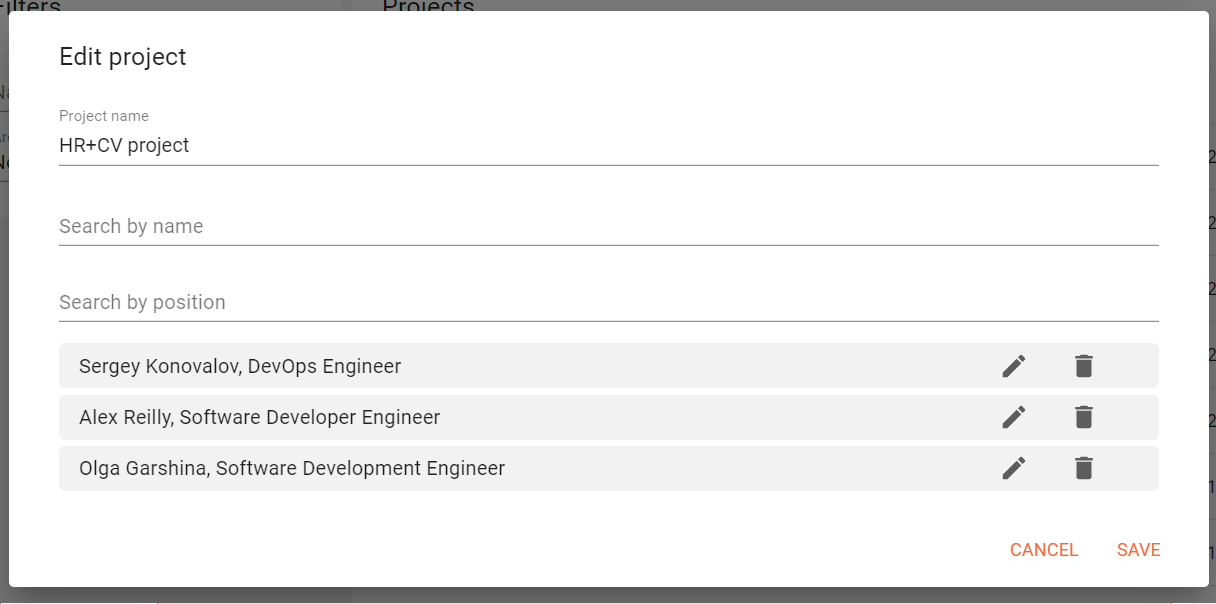
\includegraphics[width=1\textwidth]{resources/editProject.png}
\caption{Подобие папки проекта}
\label{18}
\end{figure}

Коллекция ролей имеет важную роль для создания резюме. Сами роли — это фиксированное количество терминов около 20-ти штук, от которых зависит заполнение резюме.
Так, например, на рисунке показана роль разработчика-тестировщика, для которого важно сначала отображать технологии из разряда языков программирования, после из сферы тестирования и так далее.
Приоритет категорий можно менять местами, для этого реализован так называемый drug-and-drop компонент (рис. ~\ref{19}).

\begin{figure}[!ht]
\centering
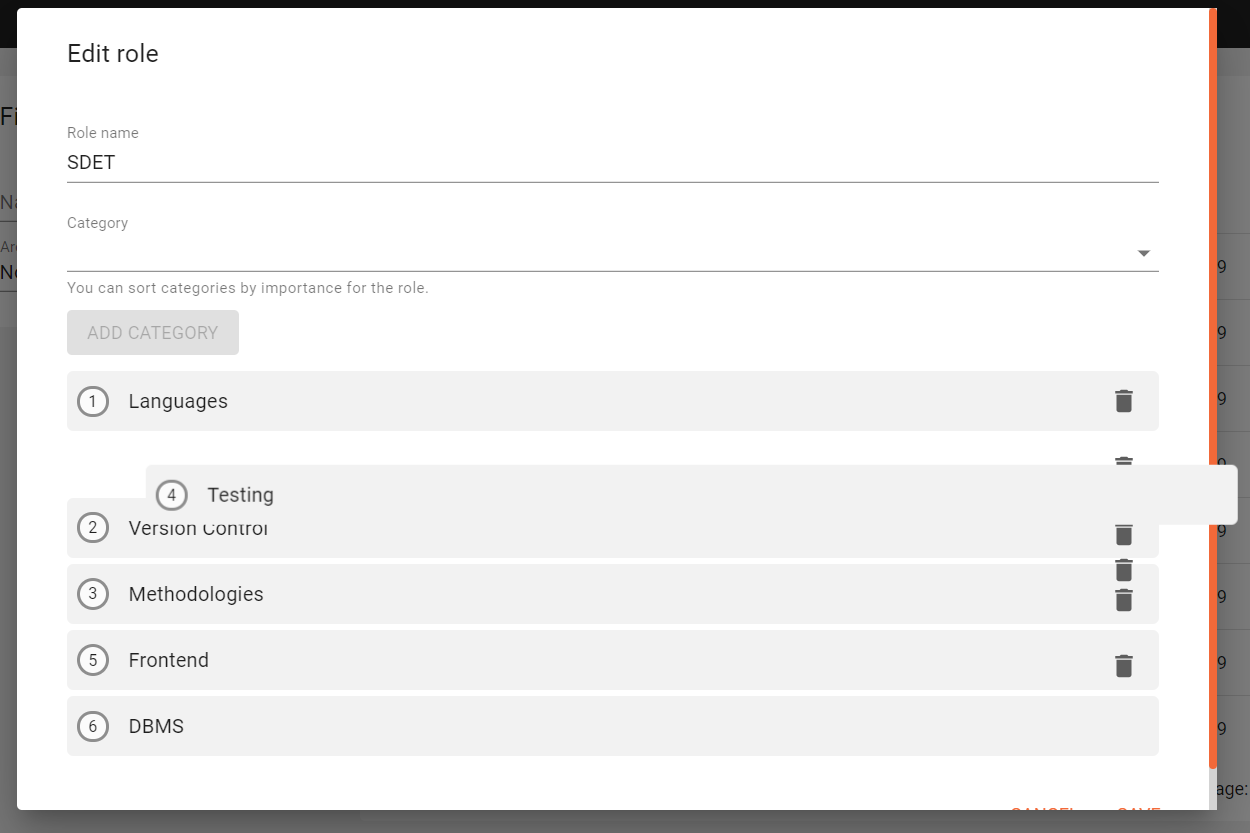
\includegraphics[width=1\textwidth]{resources/roles.png}
\caption{Перетаскивание категории testing на вторую позицию}
\label{19}
\end{figure}

В коллекции skills к каждому навыку привязан массив из "деталей". Это короткие предложения, которые раскрывают суть навыка и предлагаются пользователю при выборе конкретного умения.

Технологии отличаются тем, что они должны быть привязаны к определенной категории, иначе они автоматически будут попадать в категорию "others".

Коллекция с шаблонами выполняет одну из самых важных ролей. В ней хранятся стандартные фразы для заполнения полей типа summary, personal results и responsibilities. Чтобы словосочетание имело в себе место, выделенное жирным текстом, которое потом превратится в шаблон, рекрутеру надо просто обернуть его в угловые скобки.
Также нужно выбрать один из трех типов фразы и закрепить ее за определенной ролью.

Последняя вкладка меню отвечает за две вещи: выгрузку .docx файла, в котором содержится последняя конфигурация, описывающая все стили резюме word документа и загрузку файла с новой настроенной конфигурацией.
Было решено снова написать собственный компонент и застилизовать анимацию при Drag-and-Drop с помощью LESS. Таким образом я с нуля написала всем знакомый интерфейс (рис. ~\ref{20}), когда документ можно загрузить, просто опуская его из директории в выделенную область или кликнув по ней, чтобы открылся проводник на компьютере. Была написана валидация на формат загружаемого документа -- если пользователь пытается загрузить что-то, кроме .docx, то его предупреждает мой сервис оповещений.

\begin{figure}[!ht]
\centering

\includegraphics[width=1\textwidth]{resources/doc.png}
\caption{Интерфейс изменения конфигурации выгружаемого документа с резюме}
\label{20}
\end{figure}

\chapter{Результаты решения задачи}

В результате решения задачи было получено расширение для VSCode

\chapternonum{Заключение}

% Если нужно, меняем название Литература
\renewcommand{\bibname}{Список литературы}
\begin{thebibliography}{9}
% Если нужно сделать N. вместо [N]
% \makeatletter\renewcommand{\@biblabel}[1]{#1.}\makeatother

\bibitem{VSCode}
Visual Studio Code - Code Editing. Redefined
URL: https://code.visualstudio.com
(дата доступа: 09.06.2020)

\end{thebibliography}

\end{document}